\section{第九章\quad 气体动力循环}

% 1、2、3、4、6、7 ppt 全部

\pt{动力循环分析方法}：将复杂不可逆实际循环抽象为可逆理论循环，先找影响经济性的主要因素，再比较实际循环偏离。第一定律看能量数量，第二定律、熵分析、㶲分析看能量质量与损失。

\pt{活塞式内燃机的分类}

\begin{itemize}
    \item \pt{按燃料}：煤气机、汽油机、柴油机。
    \item \pt{按点火方式}：点燃式、压燃式。
    \item \pt{按冲程}：二冲程、四冲程。
\end{itemize}

\pt{活塞式内燃机循环特点}：实际上是开式循环；燃烧、传热、排气、膨胀、压缩等过程都存在不可逆性；各环节中工质的质量和成分会发生变化。

\pt{空气标准假设}：工质为空气，视为理想气体且定比热；燃烧简化为外部吸热，排气简化为放热；忽略燃料导致的质量、成分变化；压缩和膨胀常取等熵。

\divider

\noindent
\begin{minipage}
    [t]{0.48\linewidth}
    \vspace{0pt}
    \raggedright
    \pt{简化前的混合加热内燃机（柴油机）}：
    \begin{itemize}
        \item $0\to1$：吸气。
        \item $1\to2$：压缩。
        \item $2\to3$：喷油、定容燃烧。
        \item $3\to4$：定压燃烧。
        \item $4\to5$：膨胀作功。
        \item $5\to0$：排气。
    \end{itemize}
\end{minipage}
\hfill
\begin{minipage}
    [t]{0.48\linewidth}
    \vspace{0pt}
    \centering
    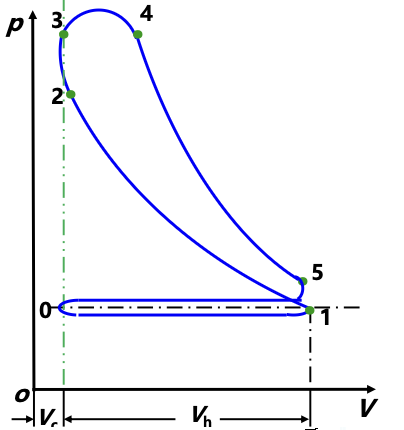
\includegraphics[width=.6\linewidth]{figures/9柴油机实际循环.png}
\end{minipage}

\noindent
\begin{minipage}
    [t]{0.35\linewidth}
    \vspace{0pt}
    \raggedright
    \pt{混合加热理想循环（萨巴德循环，柴油机）}：
    \begin{itemize}
        \item $1\to2$：等熵压缩。
        \item $2\to3$：定容吸热。
        \item $3\to4$：定压吸热。
        \item $4\to5$：等熵膨胀。
        \item $5\to1$：定容放热。
    \end{itemize}
\end{minipage}
\hfill
\begin{minipage}
    [t]{0.64\linewidth}
    \vspace{0pt}
    \centering
    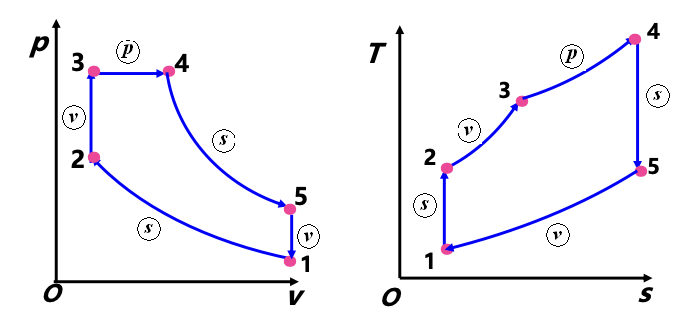
\includegraphics[width=\linewidth]{figures/9萨巴德循环.png}
\end{minipage}

\begin{itemize}
    \item \pt{循环吸热量}：$q_1=c_{\mathrm{V}}(T_3-T_2)+c_p(T_4-T_3)$，
    \item \pt{循环放热量}：$q_2=c_{\mathrm{V}}(T_5-T_1)$，
    \item \pt{热效率}：$\eta_{\mathrm{t}}=1-\frac{T_5-T_1}{(T_3-T_2)+\kappa(T_4-T_3)}$，其中 $\kappa=\frac{c_p}{c_v}$。
\end{itemize}

\pt{特性参数}

\begin{itemize}
    \item 压缩比：$\varepsilon=\frac{v_1}{v_2}$，定容增压比：$\lambda=\frac{p_3}{p_2}$，定压预胀比：$\rho=\frac{v_4}{v_3}$。
    \item \pt{等熵压缩} $1\to2$：$T_2=T_1\varepsilon^{\kappa-1}$。
    \item \pt{定容吸热} $2\to3$：$T_3=T_1\lambda\varepsilon^{\kappa-1}$。
    \item \pt{定压吸热} $3\to4$：$T_4=T_1\rho\lambda\varepsilon^{\kappa-1}$。
    \item \pt{定容放热前状态}：$T_5=T_1\lambda\rho^\kappa$。
    \item \pt{混合加热循环热效率}：$\eta_{\mathrm{t}}=1-\frac{\lambda\rho^\kappa-1}{\varepsilon^{\kappa-1}[(\lambda-1)+\kappa\lambda(\rho-1)]}$。
\end{itemize}

$\varepsilon\uparrow,\lambda\uparrow\Rightarrow\eta_{\mathrm{t}}\uparrow$；$\rho\uparrow\Rightarrow\eta_{\mathrm{t}}\downarrow$。

\divider

\noindent
\begin{minipage}
    [t]{0.35\linewidth}
    \vspace{0pt}
    \raggedright
    \pt{定压加热理想循环（狄塞尔循环，柴油机）}
    \begin{itemize}
        \item $1\to2$：等熵压缩。
        \item $2\to3$：定压吸热。
        \item $3\to4$：等熵膨胀。
        \item $4\to1$：定容放热。
    \end{itemize}
\end{minipage}
\hfill
\begin{minipage}
    [t]{0.64\linewidth}
    \vspace{0pt}
    \centering
    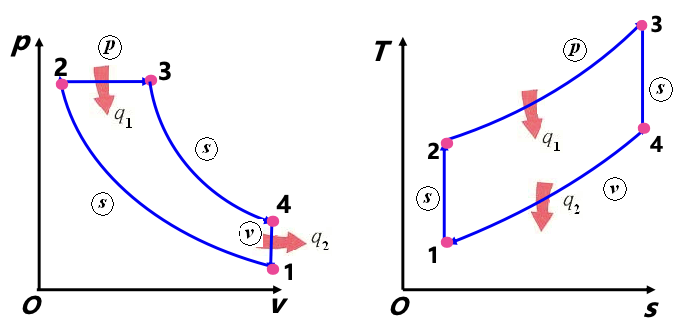
\includegraphics[width=\linewidth]{figures/9狄塞尔循环.png}
\end{minipage}

\begin{itemize}
    \item \pt{特性参数}：$\varepsilon=v_1/v_2$、$\rho=v_3/v_2$，且 $\lambda=1$。
    \item \pt{吸热量}：$q_1=c_p(T_3-T_2)$。
    \item \pt{放热量}：$q_2=c_v(T_4-T_1)$。
    \item \pt{热效率}：$\eta_{\mathrm{t}}=1-\frac{T_4-T_1}{\kappa(T_3-T_2)}$。
    \item 由混合加热循环公式令 $\lambda=1$，得 $\eta_{\mathrm{t}}=1-\frac{\rho^\kappa-1}{\kappa\varepsilon^{\kappa-1}(\rho-1)}$。
\end{itemize}

\pt{循环讨论}：
\begin{itemize}
    \item $\varepsilon$ 增大时，$\eta_{\mathrm{t}}$ 增大，$w_{\mathrm{net}}$ 增大。
    \item $\rho$ 增大时，$\eta_{\mathrm{t}}$ 降低，但 $w_{\mathrm{net}}$ 增大。
    \item 重负荷时，$\rho$ 增大、$q_1$ 增大，内部热效率下降。
    \item 温度升高会使 $\kappa$ 降低，这也是实际热效率下降的原因之一。
\end{itemize}

\divider

\pt{定容加热循环（奥托循环，汽油机）}

\begin{center}
    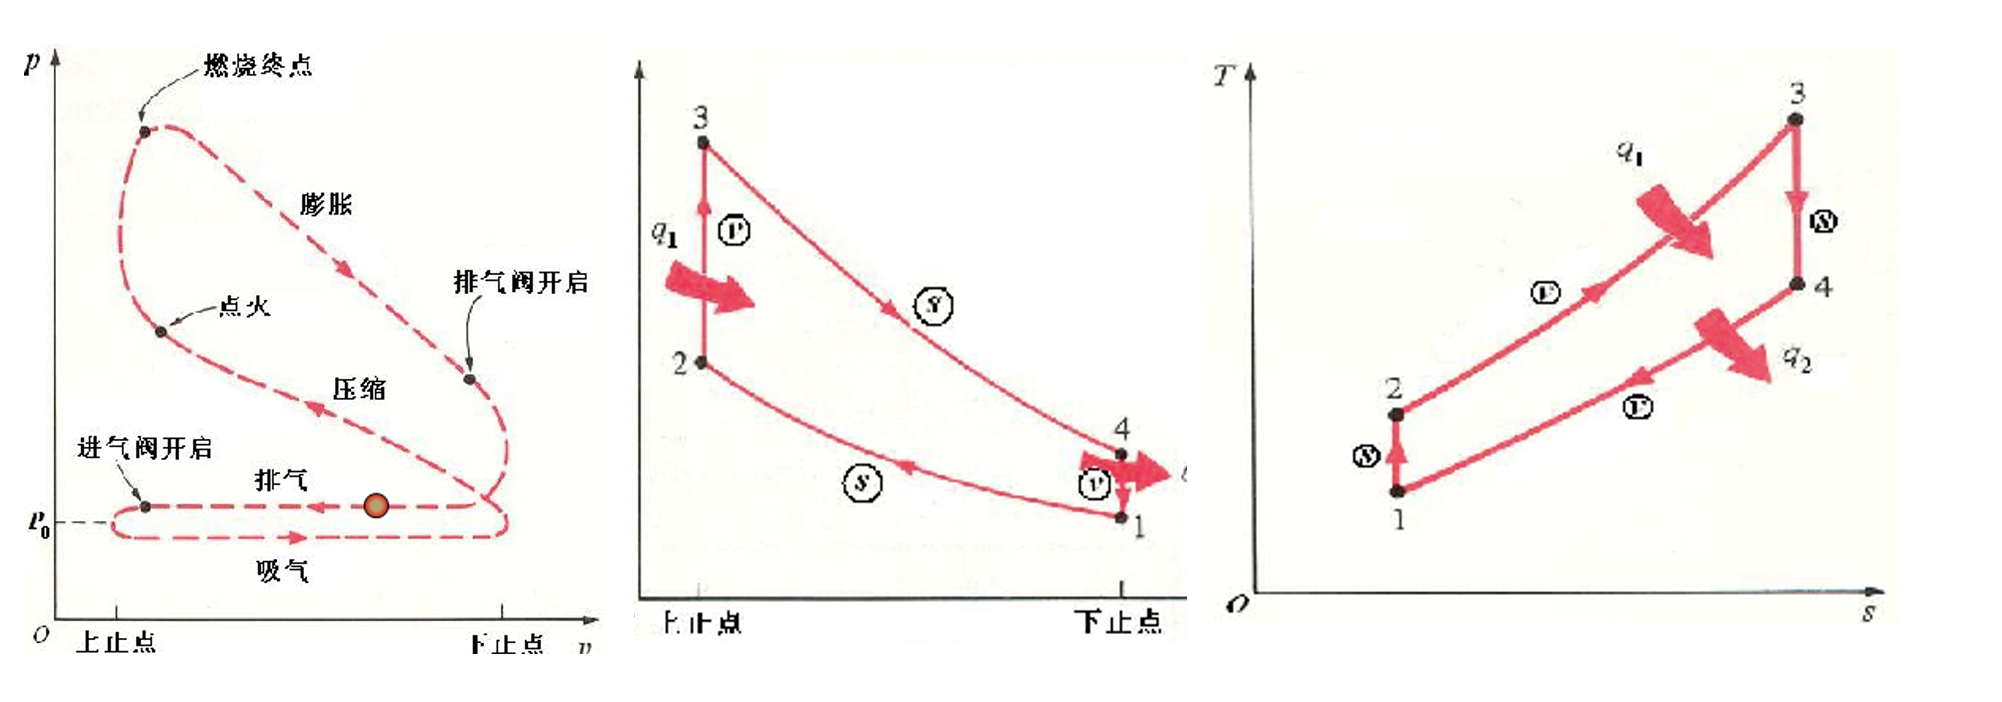
\includegraphics[width=\linewidth]{figures/9汽油机和otto循环.png}
\end{center}

\begin{itemize}
    \item $1\to2$：等熵压缩。
    \item $2\to3$：定容吸热。
    \item $3\to4$：等熵膨胀。
    \item $4\to1$：定容放热。
\end{itemize}
\par
\begin{itemize}
    \item \pt{特性参数}：$\varepsilon=v_1/v_2$、$\lambda=p_3/p_2$，且 $\rho=1$。
    \item \pt{吸热量}：$q_1=c_v(T_3-T_2)$。
    \item \pt{放热量}：$q_2=c_v(T_4-T_1)$。
    \item \pt{热效率}：$\eta_{\mathrm{t}}=1-\frac{T_4-T_1}{T_3-T_2}$。
    \item \pt{热效率}：$\eta_{\mathrm{t}}=1-\frac{1}{\varepsilon^{\kappa-1}}$。
\end{itemize}

\pt{循环讨论}：

\begin{itemize}
    \item $\varepsilon$ 增大，$\eta_{\mathrm{t}}$ 增大。
    \item $\lambda$ 增大，理想定比热条件下 $\eta_{\mathrm{t}}$ 不变，但 $w_{\mathrm{net}}$ 增大。
    \item 重负荷时，$q_1$ 增大，实际内部热效率下降，原因是温度升高导致 $\kappa$ 降低。
\end{itemize}

\divider

\pt{三种内燃机循环比较}：

\noindent
\begin{minipage}
    [t]{0.35\linewidth}
    \vspace{0pt}
    \raggedright
    \pt{压缩比相同、吸热量相同时}
    \begin{itemize}
        \item 三类循环满足 $q_{1v}=q_{1m}=q_{1p}$。
        \item 放热量关系为 $q_{2v}<q_{2m}<q_{2p}$。
        \item $\eta_{\mathrm{t}}=1-q_2/q_1$，$\eta_{\mathrm{t},v}>\eta_{\mathrm{t},m}>\eta_{\mathrm{t},p}$。
    \end{itemize}
\end{minipage}
\hfill
\begin{minipage}
    [t]{0.64\linewidth}
    \vspace{0pt}
    \centering
    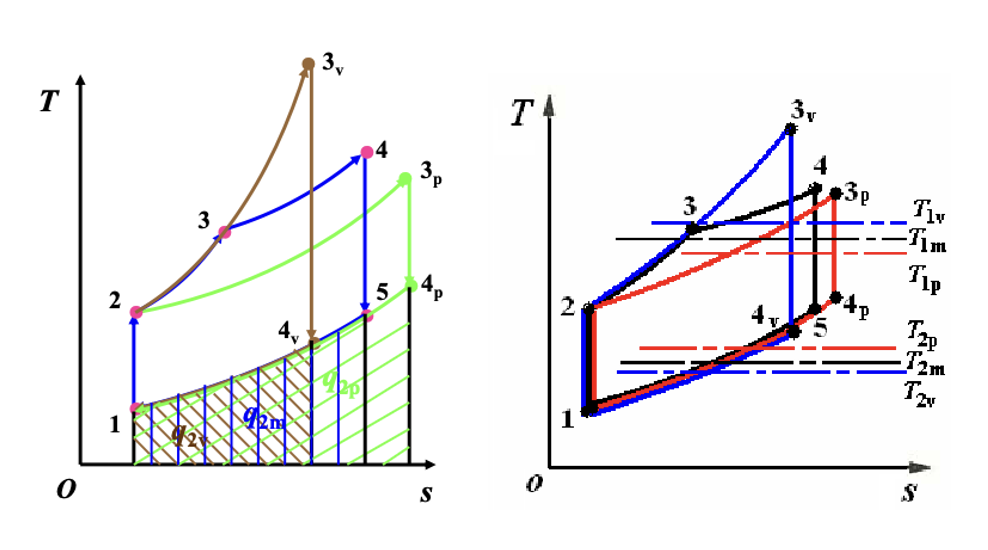
\includegraphics[width=\linewidth]{figures/9等压缩比等吸热.png}
\end{minipage}

\begin{itemize}
    \item $v$ 表示定容加热循环，$m$ 表示混合加热循环，$p$ 表示定压加热循环。
\end{itemize}

%\newcolumn

\noindent
\begin{minipage}
    [t]{0.64\linewidth}
    \vspace{0pt}
    \raggedright
    \pt{循环最高压力 $p_{\max}$ 和最高温度 $T_{\max}$ 相同时}
    \begin{itemize}
        \item $q_{2p}=q_{2m}=q_{2v}$。
        \item 吸热量关系为 $q_{1p}>q_{1m}>q_{1v}$。
        \item 因此 $\eta_{\mathrm{t},p}>\eta_{\mathrm{t},m}>\eta_{\mathrm{t},v}$。
    \end{itemize}
\end{minipage}
\hfill
\begin{minipage}
    [t]{0.35\linewidth}
    \vspace{0pt}
    \centering
    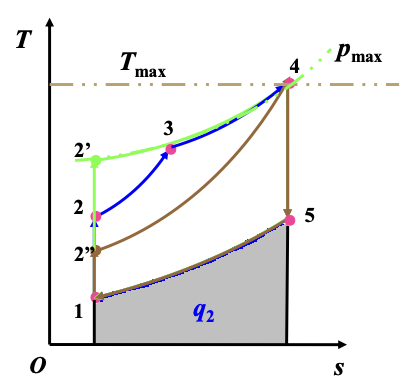
\includegraphics[width=.8\linewidth]{figures/9同最高压最高温.png}
\end{minipage}


\divider

\pt{燃气轮机装置主要构成}：压气机、燃烧室、气轮机。

\pt{燃气轮机装置特点}：实际为开式循环，工质在设备间连续流动；运转平稳，可连续输出功；启动快，到达满负荷快；压气机耗功很大，消耗气轮机产生功率的绝大部分，但装置功率重量比仍较大。

\pt{主要用途}：飞机动力、舰船动力、电站峰荷机组。

\pt{空气标准假设}：
\begin{itemize}
    \item 工质为空气，满足理想气体状态方程。
    \item 比热容取定值。
    \item 压缩和膨胀简化为等熵过程。
    \item 燃烧简化为定压吸热，排气简化为定压放热。
    \item 忽略燃油质量及燃气成分变化。
\end{itemize}

\pt{空气标准燃气轮机循环}：在上述假设下，实际开式燃气轮机循环可简化为闭式定压加热循环。

\pt{布雷顿循环（燃气轮机理想循环）}

\noindent
\begin{minipage}
    [t]{0.35\linewidth}
    \vspace{0pt}
    \raggedright
    \begin{itemize}
        \item $1\to2$：压气机内等熵压缩。
        \item $2\to3$：燃烧室内定压吸热。
        \item $3\to4$：气轮机内等熵膨胀。
        \item $4\to1$：定压放热。

    \end{itemize}
\end{minipage}
\hfill
\begin{minipage}
    [t]{0.64\linewidth}
    \vspace{0pt}
    \centering
    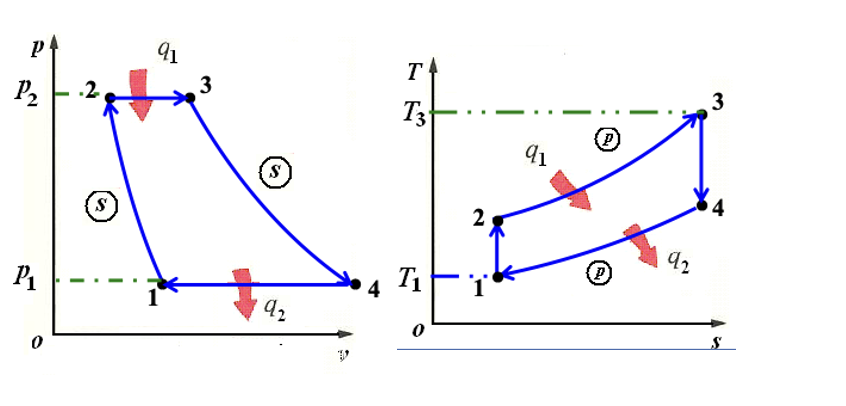
\includegraphics[width=\linewidth]{figures/9布雷顿循环.png}
\end{minipage}

\pt{循环增压比} $\pi=p_2/p_1$。\pt{循环增温比} $\tau=T_3/T_1$。

\pt{循环分析}

\begin{itemize}
    \item \pt{吸热量} $q_1=h_3-h_2=c_p(T_3-T_2)$。
    \item \pt{放热量} $q_2=h_4-h_1=c_p(T_4-T_1)$。
    \item \pt{热效率} $\eta_{\mathrm{t}}=1-\frac{q_2}{q_1}=1-\frac{T_4-T_1}{T_3-T_2}=1-\frac{T_1}{T_2}=1-\frac{1}{\pi^{(\kappa-1)/\kappa}}$。
    \item 注意：式中的 $T_1$、$T_2$ 是循环状态点温度，不是高温热源和低温热源温度。
\end{itemize}

\pt{循环分析}

\begin{itemize}
    \item $\pi$ 增大，$\eta_{\mathrm{t}}$ 增大。
    \item 理想定比热条件下，$\eta_{\mathrm{t}}$ 与循环最高温度 $T_3$ 无关。
    \item 当 $\pi$ 一定时，增大 $\tau$ 可增大吸热量和净功，但热效率不变。
    \item 循环净功为 $w_{\mathrm{net}}=c_p[(T_3-T_2)-(T_4-T_1)]$。
    \item 令 $r=\pi^{(\kappa-1)/\kappa}$，则 $w_{\mathrm{net}}=c_pT_1(r-1)(\tau/r-1)$。
    \item 当 $\tau$ 一定时，存在使 $w_{\mathrm{net}}$ 最大的最佳增压比。
    \item 最大净功条件为 $\pi=\tau^{\kappa/[2(\kappa-1)]}$。
    \item $\tau$ 升高，即 $T_3$ 升高，会使取得 $w_{\mathrm{net,max}}$ 的 $\pi$ 升高，并使 $\eta_{\mathrm{t}}$ 和 $w_{\mathrm{net,max}}$ 同时升高。
\end{itemize}

\divider

\noindent
\begin{minipage}
    [t]{0.64\linewidth}
    \vspace{0pt}
    \raggedright
    \pt{实际布雷顿循环}
    \begin{itemize}
        \item $1\to2$：不可逆绝热压缩。
        \item $2\to3$：定压吸热。
        \item $3\to4$：不可逆绝热膨胀。
        \item $4\to1$：定压放热。
    \end{itemize}
\end{minipage}
\hfill
\begin{minipage}
    [t]{0.35\linewidth}
    \vspace{0pt}
    \centering
    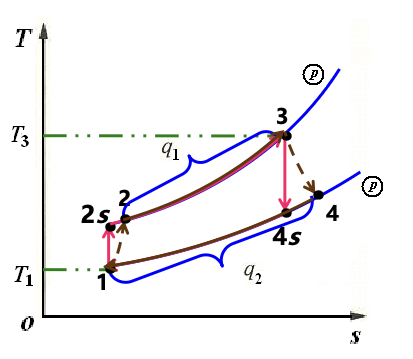
\includegraphics[width=.8\linewidth]{figures/9实际布雷顿循环.png}
\end{minipage}

\pt{压气机绝热效率}：
\begin{itemize}
    \item $\eta_{\mathrm{C,s}}=w_{\mathrm{C,s}}/w_{\mathrm{C}}'=\frac{h_{2s}-h_1}{h_2-h_1}$。
    \item 因此 $h_2=h_1+\frac{h_{2s}-h_1}{\eta_{\mathrm{C,s}}}$。
\end{itemize}
\pt{燃气轮机相对内效率}：
\begin{itemize}
    \item $\eta_{\mathrm{T}}=w_{\mathrm{t,T}}'/w_{\mathrm{t,T}}=\frac{h_3-h_4}{h_3-h_{4s}}$。
    \item 因此 $h_4=h_3-\eta_{\mathrm{T}}(h_3-h_{4s})$。
\end{itemize}
\pt{内部热效率}：
\begin{itemize}
    \item $\eta_{\mathrm{i}}=w_{\mathrm{net}}'/q_1'$。
    \item 实际净功为 $w_{\mathrm{net}}'=\eta_{\mathrm{T}}(h_3-h_{4s})-\frac{h_{2s}-h_1}{\eta_{\mathrm{C,s}}}$。
    \item 实际吸热量为 $q_1'=h_3-h_2=h_3-h_1-\frac{h_{2s}-h_1}{\eta_{\mathrm{C,s}}}$。
    \item 令 $r=\pi^{(\kappa-1)/\kappa}$，可写为 $\eta_{\mathrm{i}}=\frac{\eta_{\mathrm{T}}\tau(1-1/r)-(r-1)/\eta_{\mathrm{C,s}}}{\tau-1-(r-1)/\eta_{\mathrm{C,s}}}$。
\end{itemize}

\pt{循环讨论}

\begin{itemize}
    \item $\eta_{\mathrm{i}}$ 与 $\pi$、$\tau$ 有关。
          \subitem $\pi$ 一定时，$\tau$ 增大，$\eta_{\mathrm{i}}$ 增大。
          \subitem $\tau$ 一定时，$\pi$ 增大，$\eta_{\mathrm{i}}$ 会变化并存在极值。
    \item $\eta_{\mathrm{i}}$ 与 $\eta_{\mathrm{T}}$ 和 $\eta_{\mathrm{C,s}}$ 有关。
          \subitem $\eta_{\mathrm{T}}$ 增大、$\eta_{\mathrm{C,s}}$ 增大，会使 $\eta_{\mathrm{i}}$ 增大。
          \subitem 典型范围为 $\eta_{\mathrm{T}}=0.85\sim0.92$
          \subitem $\eta_{\mathrm{C,s}}=0.85\sim0.90$。
    \item 增大 $\tau$ 是提高燃气轮机装置性能，即提高 $w_{\mathrm{net}}$ 和 $\eta_{\mathrm{i}}$ 的重要方向。
\end{itemize}

\divider

\noindent
\begin{minipage}
    [t]{0.64\linewidth}
    \vspace{0pt}
    \raggedright
    \pt{回热}：利用燃气轮机排气预热压气机出口空气，减少燃烧室吸热。空气先被废气预热到 $T_5$，燃烧室只需要从 $T_5$ 加热到 $T_3$，吸热量为
    $q_1'=c_p(T_3-T_5)$\\
    \begin{itemize}
        \item $5$ 点：压气机出口空气在极限回热情况下能被预热到的最高状态 $T_5=T_4$
        \item $6$ 点：气轮机排气在极限回热情况下放热后能降到的最低状态 $T_6=T_2$
    \end{itemize}

\end{minipage}
\hfill
\begin{minipage}
    [t]{0.35\linewidth}
    \vspace{0pt}
    \centering
    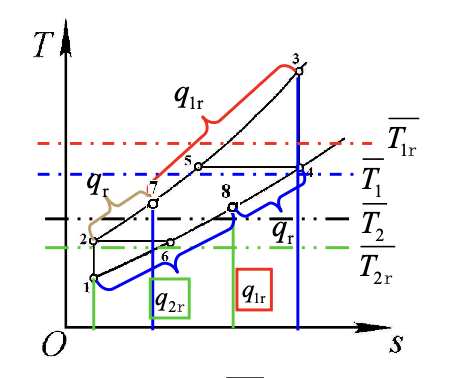
\includegraphics[width=\linewidth]{figures/9回热.png}
\end{minipage}

\begin{itemize}
    \item $7$ 点：实际回热后，压气机出口空气被预热后的状态。
    \item $8$ 点：实际回热后，气轮机排气放热后的状态。
\end{itemize}

\pt{回热度} $\sigma=\frac{\text{实际回热利用的热量}}{\text{理论极限可利用的热量}}=\frac{h_7-h_2}{h_5-h_2}=\frac{h_4-h_8}{h_4-h_6}$；

\pt{极限回热} $q_{1r}=c_p(T_3-T_5)$，$q_{2r}=c_p(T_6-T_1)$。需 $T_4>T_2$ 才有有效温差。

\noindent
\begin{minipage}
    [t]{0.7\linewidth}
    \vspace{0pt}
    \raggedright
    \pt{实际循环回热} $\sigma'=\frac{h_7-h_{2'}}{h_5-h_{2'}}$。
\end{minipage}
\hfill
\begin{minipage}
    [t]{0.29\linewidth}
    \vspace{0pt}
    \centering
    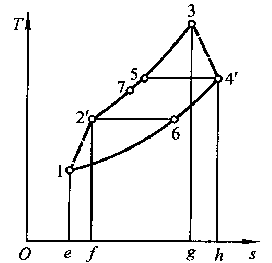
\includegraphics[width=\linewidth]{figures/9实际回热.png}
\end{minipage}

理想回热效率 $\eta_{\mathrm{t,r}}=1-\frac{q_{2r}}{q_{1r}}$，
通常 $\eta_{\mathrm{t},r}>\eta_{\mathrm{t}}$。

\divider

\pt{分级压缩中冷}：降低压气机耗功，但单独用于简单布雷顿循环时，因压气机出口温度降低、需补充更多热量，热效率不一定提高；若与回热结合，中冷增大可回热温差，可提高热效率。

\pt{分级膨胀再热}：可增加燃气轮机输出功；无回热时可能降低热效率；与回热结合时因排气温度提高、回热效果增强，可提高热效率。分级压缩中冷、分级膨胀再热和回热联合，级数趋于无穷时趋近概括性卡诺循环。

\divider
